% ---------
% --------
%!TEX TS-program = pdflatex
%!TEX encoding = UTF-8 Unicode
%!TEX spellcheck = English (Aspell)

\documentclass[11pt]{article}
\usepackage{lucy,handout,graphicx}
\usepackage{fourier-orns}
\usepackage{mathtools}
\usepackage[normalem]{ulem} % either use this (simple) or
\usepackage{tikz}
\usetikzlibrary{graphs}

\allowdisplaybreaks


\begin{document}

\noindent Name \underline{\hspace{12cm}}\\

\begin{center}
\Large\textbf{CSCI 332, Fall 2026}\\
\LARGE\textbf{Exam 1 Collected Problems}
\end{center}

\noindent This practice exam collects the problems on the following topics from
 the Fall 2025 exams, practice exams, and final exam:
\begin{enumerate}
    \item Stable Matching
    \item Algorithm Analysis
    \item Recursion
    \item 1D Dynamic Programming
\end{enumerate}

Problems are grouped by topic and labeled with their source exam. Original
point values, where provided, are retained for reference; this collection is
not a single 100-point exam. Repeated problems and variants from the source
exams are included.

If you need more space than what is given, use additional scratch paper.

Good luck!

\newpage

\begin{center}
\LARGE\textbf{Section 1 (Stable Matching)\\}%
\end{center}

% Source: cs332-fall2025/exams/exam1/main.tex
\subsection*{From Fall 2025 Exam 1}
\begin{enumerate}
\item (7 points) The input to the \emph{stable
matching problem} is a set of $n$ men, a set of $n$ women, and preference lists
ranking each man for each woman and each woman for each man. Describe the
desired output as precisely as you can.

\vspace{1in}

A matching for the following preference lists for 4 men and 4 women is given by
the capitalized men and women.

\begin{center}
\begin{tabular}{ c c c }
    $m_1$: $w_1$, $w_4$, $w_3$, $W_2$ &  $w_1$: $m_4$, $m_3$, $M_2$, $m_1$\\
    $m_2$: $W_1$, $w_3$, $w_2$, $w_4$ &  $w_2$: $m_4$, $m_2$, $M_1$, $m_3$\\
    $m_3$: $w_4$, $w_1$, $W_3$, $w_2$ &  $w_3$: $m_1$, $M_3$, $m_2$, $m_4$\\ 
    $m_4$: $W_4$, $w_3$, $w_2$, $w_1$ &  $w_4$: $m_3$, $m_1$, $m_2$, $M_4$
\end{tabular}
\end{center}

    
    \item (5 points) Is this matching stable? Yes or no

    \item (5 points) How do you know?

\vspace{1in}


\item (8 points)
This is the same preference list for 4 men and 4 women given above.

\begin{center}
\begin{tabular}{ c c c }
    $m_1$: $w_1$, $w_4$, $w_3$, $w_2$ &  $w_1$: $m_4$, $m_3$, $m_2$, $m_1$\\
    $m_2$: $w_1$, $w_3$, $w_2$, $w_4$ &  $w_2$: $m_4$, $m_2$, $m_1$, $m_3$\\
    $m_3$: $w_4$, $w_1$, $w_3$, $w_2$ &  $w_3$: $m_1$, $m_3$, $m_2$, $m_4$\\ 
    $m_4$: $w_4$, $w_3$, $w_2$, $w_1$ &  $w_4$: $m_3$, $m_1$, $m_2$, $m_4$
\end{tabular}
\end{center}

 What is the outcome of the Gale-Shapley algorithm on this input? Assume that men propose to women.
\vspace{1in}



\item (5 points) True or false? In every instance of the
 Stable Matching Problem, there is a stable matching containing a pair $(m,w)$
 such that $m$ is ranked first on the preference list of $w$ and $w$ is ranked
 first on the preference list of $m$.


\newpage

% Source: cs332-fall2025/exams/exam1_practice1/main.tex
\subsection*{From Fall 2025 Exam 1 Practice 1}
\item (5 points) The input to the \emph{stable
matching problem} is a set of $n$ men, a set of $n$ women, and preference lists
ranking each man for each woman and each woman for each man. Describe the
desired output as precisely as you can.

\vspace{1in}

\item A matching for the following preference lists for 4 men and 4 women is given by
the capitalized men and women.

\begin{center}
\begin{tabular}{ c c c }
    $m_1$: $w_3$, $W_1$, $w_2$, $w_4$ &  $w_1$: $m_4$, $m_3$, $m_2$, $M_1$\\
    $m_2$: $W_4$, $w_1$, $w_2$, $w_3$ &  $w_2$: $M_4$, $m_3$, $m_2$, $m_1$\\
    $m_3$: $w_2$, $w_1$, $W_3$, $w_4$ &  $w_3$: $m_1$, $m_2$, $m_4$, $M_3$\\ 
    $m_4$: $w_1$, $W_2$, $w_3$, $w_4$ &  $w_4$: $m_1$, $m_3$, $m_4$, $M_2$
\end{tabular}
\end{center}

    
    \item (3 points) Is this matching stable? Yes or no

    \item (2 points) How do you know?

\vspace{1in}


\item (5 points)
This is the same preference list for 4 men and 4 women given above.

\begin{center}
\begin{tabular}{ c c c }
    $m_1$: $w_3$, $w_1$, $w_2$, $w_4$ &  $w_1$: $m_4$, $m_3$, $m_2$, $m_1$\\
    $m_2$: $w_4$, $w_1$, $w_2$, $w_3$ &  $w_2$: $m_4$, $m_3$, $m_2$, $m_1$\\
    $m_3$: $w_2$, $w_1$, $w_3$, $w_4$ &  $w_3$: $m_1$, $m_2$, $m_4$, $m_3$\\ 
    $m_4$: $w_3$, $w_2$, $w_1$, $w_4$ &  $w_4$: $m_1$, $m_3$, $m_4$, $m_2$
\end{tabular}
\end{center}

 What is the outcome of the Gale-Shapley algorithm on this input? Assume that men propose to women.
\vspace{1in}

\item (5 points) True or false? In every instance of the
 Stable Matching Problem, there is a stable matching containing a pair $(m,w)$
 such that $m$ is ranked first on the preference list of $w$ and $w$ is ranked
 first on the preference list of $m$.


\newpage

% Source: cs332-fall2025/exams/exam1_practice2/main.tex
\subsection*{From Fall 2025 Exam 1 Practice 2}
Recall the Gale-Shapley Algorithm for solving the stable matching problem:

    \begin{algo}
    Gale-Shapley(preference lists for $n$ hospitals and $n$ students)\+\\
    Let $M$ be an empty matching\\
    While some hospital $h$ is umatched and hasn't proposed to every student:\+ \\
        Let $s$ be the first student on $h$'s list to whom $h$ has not yet proposed\\
        If $s$ is unmatched:\+\\
            Add $(h,s)$ to $M$\-\\
        Else $s$ is matched to $h'$:\+\\
            If $s$ prefers $h$ to $h'$:\+\\
                Remove $(h',s)$ from $M$\\
                Add $(h,s)$ to $M$\-\\
            Else $s$ prefers $h'$ to $h$:\+\\
                Do nothing\-\-\-\\
    Return $M$\\
    \end{algo}



\item (10 points) For each of the following claims about the Gale-Shapley
algorithm on any input, mark whether they are true or false. 
\begin{enumerate}[(a)]
    \item Once a hospital becomes matched, it never becomes unmatched. T or F
    \item Once a student becomes matched, it never becomes unmatched. T or F
\end{enumerate}

\item (5 points)
Describe a best-case input for the Gale-Shapley algorithm.

\vspace{1in}

\item (10 points) Give the smallest, simplest function $f(n)$ that you can such
that the the number of iterations of the while loop in the Gale-Shapley
algorithm is $O(f(n))$ on any input of $n$ hospitals and $n$ students. 

\vspace{1in}

\item (5 points) Write the name or definition of the following set symbols:
    \begin{enumerate}[(a)]
        \item $\subseteq$:
        \item $\cup$:
        \item $\cap$:
        \item $\mathcal{P}$:
        \item $\in$:
    \end{enumerate}



\newpage
% Source: cs332-fall2025/exams/final/sections/stable_matching.tex
\subsection*{From Fall 2025 Final Exam}

\item Is $\{(h_1, s_4), (h_2, s_1), (h_3, s_3), (h_4, s_2)\}$ a stable matching for the given preference lists?

\begin{table}[h]
\centering
\begin{tabular}{c | l || c | l}
\textbf{Hospital} & \textbf{Preferences} & \textbf{Student} & \textbf{Preferences} \\
\hline
$h_1$ & $s_2 , s_3 , s_4 , s_1$ & $s_1$ & $h_3 , h_1 , h_2 , h_4$ \\
$h_2$ & $s_1 , s_3 , s_2 , s_4$ & $s_2$ & $h_2 , h_3 , h_4 , h_1$ \\
$h_3$ & $s_3 , s_4 , s_2 , s_1$ & $s_3$ & $h_3 , h_2 , h_4 , h_1$ \\
$h_4$ & $s_1 , s_3 , s_2 , s_4$ & $s_4$ & $h_4 , h_1 , h_3 , h_2$ \\
\end{tabular}
\end{table}

Select A for yes and B for no.

\item Given the matching
$\{(h_4, s_1), (h_1, s_3), (h_3, s_4), (h_2, s_2)\}$ and the
preference lists below,
select all unstable pairs from the list.

\begin{table}[h]
\centering
\begin{tabular}{c | l || c | l}
\textbf{Hospital} & \textbf{Preferences} & \textbf{Student} & \textbf{Preferences} \\
\hline
$h_1$ & $s_1 , s_2 , s_3 , s_4$ & $s_1$ & $h_3 , h_2 , h_1 , h_4$ \\
$h_2$ & $s_1 , s_2 , s_4 , s_3$ & $s_2$ & $h_1 , h_2 , h_3 , h_4$ \\
$h_3$ & $s_2 , s_1 , s_3 , s_4$ & $s_3$ & $h_1 , h_3 , h_4 , h_2$ \\
$h_4$ & $s_4 , s_2 , s_3 , s_1$ & $s_4$ & $h_3 , h_4 , h_2 , h_1$ \\
\end{tabular}
\end{table}

\begin{enumerate}[A.]
    \item $(h_4, s_1)$
    \item $(h_2, s_4)$
    \item $(h_2, s_1)$
    \item $(h_3, s_3)$
    \item $(h_1, s_2)$
\end{enumerate}


The following questions refer to the Gale-Shapley algorithm for
stable matching.

    \begin{algo}
    Gale-Shapley(preference lists for $n$ hospitals and $n$ students)\+\\
    Let $M$ be an empty matching\\
    While some hospital $h$ is umatched and hasn't proposed to every student:\+ \\
        Let $s$ be the first student on $h$'s list to whom $h$ has not yet proposed\\
        If $s$ is unmatched:\+\\
            Add $(h,s)$ to $M$\-\\
        Else $s$ is matched to $h'$:\+\\
            If $s$ prefers $h$ to $h'$:\+\\
                Remove $(h',s)$ from $M$\\
                Add $(h,s)$ to $M$\-\\
            Else $s$ prefers $h'$ to $h$:\+\\
                Do nothing\-\-\-\\
    Return $M$\\
    \end{algo}

\item Does the Gale-Shapley algorithm always terminate with a stable matching?
Select A for yes and B for no.

\item Are there inputs for which the Gale-Shapley algorithm runs in $O(n)$ time?
Select A for yes and B for no.

\item Are there inputs for which the Gale-Shapley algorithm runs in $O(n^2)$ time?
Select A for yes and B for no.

\item Are there inputs for which the Gale-Shapley algorithm runs in $O(n^3)$ time?
Select A for yes and B for no.

\item What is the stable matching returned by the Gale-Shapley algorithm on the
following preference list?

\begin{table}[h]
\centering
\begin{tabular}{c | l || c | l}
\textbf{Hospital} & \textbf{Preferences} & \textbf{Student} & \textbf{Preferences} \\
\hline
$h_1$ & $s_1 , s_2 , s_3 , s_4$ & $s_1$ & $h_3 , h_2 , h_1 , h_4$ \\
$h_2$ & $s_1 , s_2 , s_4 , s_3$ & $s_2$ & $h_1 , h_2 , h_3 , h_4$ \\
$h_3$ & $s_2 , s_1 , s_3 , s_4$ & $s_3$ & $h_1 , h_3 , h_4 , h_2$ \\
$h_4$ & $s_4 , s_2 , s_3 , s_1$ & $s_4$ & $h_3 , h_4 , h_2 , h_1$ \\
\end{tabular}
\end{table}

\begin{enumerate}[A.]
    \item $\{(h_1, s_1), (h_2, s_1), (h_3, s_2), (h_4, s_4)\}$
    \item $\{(h_1, s_1), (h_2, s_2), (h_3, s_3), (h_4, s_4)\}$
    \item $\{(h_1, s_4), (h_2, s_3), (h_3, s_1), (h_4, s_2)\}$
    \item $\{(h_1, s_2), (h_2, s_3), (h_3, s_1), (h_4, s_4)\}$
    \item $\{(h_1, s_3), (h_2, s_1), (h_3, s_4), (h_4, s_2)\}$
\end{enumerate}
\newpage

\begin{center}
\LARGE\textbf{Section 2 (Algorithm Analysis)\\}%
\end{center}

% Source: cs332-fall2025/exams/exam1/main.tex
\subsection*{From Fall 2025 Exam 1}
\item (10 points)
Suppose you have algorithms with the following runtimes.
(Assume these are exact running times as a function of the input size $n$, not
asymptotic running times.) How much slower do these algorithms get when you
double the input size? (You can find this by dividing the runtime on $2n$ by the
runtime on $n$). You should simplify your answer as much as possible, including evaluating
logarithms when possible.

\begin{enumerate}[(a)]
    \item $3n^2$ 
\vspace{1in}
    \item $\log_2 n$
\vspace{1in}
    \item $3^{n}$
\vspace{1in}
\end{enumerate}


\item (5 points) Give a function $f(n)$ such that the worst-case runtime of the following algorithm is $\Theta(f(n))$. 

    \begin{algo}
    Algorithm-1(array $A$ of length $n$):\+\\
    Result = 0\\
    For each $i$ in $1$ to $n$:\+\\
    For each $j$ in $1$ to $i$:\+\\
    Set Result to $A[j]$ times Result\-\- \\
    Return Result\\
    \end{algo} 

    \vspace{3in}

\item (10 points) 
Order the following functions from asymptotically smallest to asymptotically largest. If two functions are asymptotically
    equal (one is $\Theta$ of the other), indicate this with an equals sign. For example, if the functions were $n$, $n^2$, and $3n + 4$, the answer would be
    $n = 3n + 4 < n^2$.

    \begin{itemize}
        \item $n \log n^3$
        \item $n \log n^2$
        \item $\sqrt{n}$
        \item $n + \log n$
        \item $n^{\log_3 2}$
        \item $100^{100!}$
        \item $\log_2 n$
        \item $2^n$
        \item $3^n$
    \end{itemize}

\item (5 points) 
Suppose you know that an algorithm has a worst-case runtime that is $O(n^2 \log n)$. For each of the following, decide whether it is definitely true, definitely false, or could be true or false and circle your choice. 

\begin{itemize}
    \item The algorithm's worst-case runtime is $\Omega(n^2)$. T, F, T or F
    \item The algorithm's worst-case runtime is $\Omega(n^3)$. T, F, T or F
    \item The algorithm's best-case runtime is $O(n^2)$. T, F, T or F
    \item The algorithm's worst-case runtime is $O(n^3)$. T, F, T or F
    \item The algorithm's worst-case runtime is $\Theta(n^2 \log n)$. T, F, T or F
\end{itemize}


\newpage

% Source: cs332-fall2025/exams/exam1_practice1/main.tex
\subsection*{From Fall 2025 Exam 1 Practice 1}
\item (10 points)
For each of the following statements, circle T if it is true and F if it is false.

\begin{itemize}
    \item $2^n$ is $O(n!)$: T or F
    \item $n^3$ is $\Omega(n^2)$: T or F
    \item $n \log n$ is $\Theta(n^2)$: T or F
    \item There is an algorithm with worst-case runtime that is $\Omega(n^2)$ and best-case runtime that is $\Omega(n \log n)$: T or F
    \item There is an algorithm with worst-case runtime that is $O(n^2)$ and best-case runtime that is $\Theta(n^3)$: T or F
\end{itemize}

\item (5 points) Give a function $f(n)$ such that the worst-case runtime of the following algorithm is $\Theta(f(n))$. 

    \begin{algo}
    Algorithm-1(array $A$ of length $n$):\+\\
    Result = 0\\
    For every third $i$ in $1$ to $n$:\+\\
    For $j$ in $1$ to $i$:\+\\
    Set Result to $A[j]$ times Result\-\- \\
    Return Result\\
    \end{algo} 

    \vspace{1in}

\item (5 points) 
For the same algorithm above, give a function $g(n)$ such that the best-case
runtime of the algorithm is $\Theta(g(n))$.


\newpage

% Source: cs332-fall2025/exams/exam1_practice2/main.tex
\subsection*{From Fall 2025 Exam 1 Practice 2}
\item (5 points)
Evaluate the following:

\begin{enumerate}[(a)]
    \item $\log_2(16) = $ 
    \item $2^{\log_2(123456789)} = $
\end{enumerate}

\item (15 points) Recall the definition of big O: a function $f(n)$ is $O(g(n))$ if there
exist constants $c > 0$ and $n_0 \geq 1$ such that for every $n \geq n_0$, $f(n)
\leq c g(n)$.

Use this definition to prove that $3n^2 + 5n + 10$ is $O(n^2)$.

\vspace{3in}

\item (10 points) Give a function $f(n)$ such that the worst-case runtime of the following algorithm is $\Theta(f(n))$. 
 Recall that $\lfloor x \rfloor$ takes the \emph{floor} of $x$, meaning that it rounds down to the nearest integer.

    \begin{algo}
    Algorithm-1(array $A$ of length $n$):\+\\
    Result = 0\\
    For $i$ in $1$ to $n$:\+\\
    If $A[i]$ is even:\+\\
    For $j$ in $i + \lfloor n/2 \rfloor$ to $n$:\+\\
    Add $A[j]$ to Result\-\-\- \\
    Return Result
    \end{algo}



\newpage
% Source: cs332-fall2025/exams/final/sections/algorithm_analysis.tex
\subsection*{From Fall 2025 Final Exam}

\item Recall that the definition of big O is as follows:
\emph{$f(n)$ is $O(g(n))$ if there exist positive constants $c$ and $n_0$ such
that for all $n >= n_0$, $f(n) \leq c \cdot g(n)$.} Which $n_0$ and $c$ can be
used to show that $9n^2 + n + 10$ is $O(n^3)$?
\begin{enumerate}[A.]
    \item $n_0 = 1$, $c = 4$
    \item $n_0 = 1$, $c = 10$
    \item $n_0 = 1$, $c = 1000$
    \item $n_0=10, c = 4$
    \item $n_0 = 100$, $c = 1$

\end{enumerate}

\item Select all of the true statements below.
\begin{enumerate}[A.]
    \item $\log(100 \cdot n^{5n})$ is $\Theta(n \log n)$
    \item $\log(100 \cdot n^{5n})$ is $\Theta(n^n)$
    \item $\log(100 \cdot n^{5n})$ is $\Theta(5^n)$
    \item $\log(100 \cdot n^{5n})$ is $\Theta(n^n \log n)$
    \item $\log(100 \cdot n^{5n})$ is $\Theta(n^5 \log 100)$
\end{enumerate}

\item For which of the following is it true that $f_1(n)$ is $O(f_2(n))$ and
$f_2(n)$ is $O(f_3(n))$? (That is, the functions are in increasing
order of asymptotic growth, but two or more adjacent functions may have the same
asymptotic growth rate.) There may be more than one correct answer; select all
that apply.

\begin{enumerate}[A.]
  \item $f_1 = \dfrac{n}{10^{10}} \;,\; f_2 = n^{0.6} \;,\; f_3=\log n$
  \item $f_1=\log n \;,\; f_2 = \dfrac{n}{10^{10}} \;,\; f_3 = n^{0.6}$
  \item $f_1 = n^{0.6} \;,\; f_2=\log n \;,\; f_3 = \dfrac{n}{10^{10}}$
  \item $f_1=\log n \;,\; f_2 = n^{0.6} \;,\; f_3 = \dfrac{n}{10^{10}}$
  \item $f_1 = \dfrac{n}{10^{10}} \;,\; f_2=\log n \;,\; f_3 = n^{0.6}$
\end{enumerate}

\item For which of the following is it true that $f_1(n)$ is $O(f_2(n))$ and
$f_2(n)$ is $O(f_3(n))$? (That is, the functions are in increasing
order of asymptotic growth, but two or more adjacent functions may have the same
asymptotic growth rate.) There may be more than one correct answer; select all
that apply.

\begin{enumerate}[A.]
  
  \item $f_1 = 4^n,\; f_2 = n!,\; f_3 = 3^n$
  
  \item $f_1 = 3^n,\; f_2 = 4^n,\; f_3 = n!$
  
  \item $f_1 = 3^n,\; f_2 = n!,\; f_3 = 4^n$
  
  \item $f_1 = n!,\; f_2 = 4^n,\; f_3 = 3^n$
  
  \item $f_1 = n!,\; f_2 = 3^n,\; f_3 = 4^n$
\end{enumerate}

\item Select all functions that are $\Theta(n^2)$.

\begin{enumerate}[A.]
    \item $5n^2 + 3n + 20$
    \item $n \log n$
    \item $n^2 + n \log n$
    \item $0.5 n^2 - 10 n + 2000$
    \item $n^3$

\end{enumerate}

\item Select all functions that are $\Omega(n^2)$.

\begin{enumerate}[A.]
    \item $5n^2 + 3n + 20$
    \item $n \log n$
    \item $n^2 + n \log n$
    \item $0.5 n^2 - 10 n + 2000$
    \item $n^3$

\end{enumerate}

\item Select all functions $f(n)$ such that the worst-case runtime of
Algorithm-1 below is $\Theta(f(n))$.

    \begin{algo}
    Algorithm-1(array $A$ of length $n$):\+\\
    Result = 0\\
    For each $i$ in $1$ to $n$:\+\\
    For each $j$ in $1$ to $i$:\+\\
    Set Result to $A[j]$ times Result\-\- \\
    Return Result\\
    \end{algo} 

\begin{enumerate}[A.]
    \item $n$
    \item $\log n$
    \item $n^2$
    \item $n^3$
    \item $n!$
\end{enumerate}
\newpage

\begin{center}
\LARGE\textbf{Section 3 (Recursion)\\}%
\end{center}

% Source: cs332-fall2025/exams/exam2/main.tex
\subsection*{From Fall 2025 Exam 2}
\item (10 points) Given the following (meaningless) divide and conquer algorithm,
what is the recurrence relation that describes its running time?

    \begin{algo}
    wut(integer array $A$ of length $n$): \+ \\
    if $n \leq 1$:\+\\
        return $A$\-\\
    else:\+\\
    Let $A_1, A_2, A_3$ be the first third, middle third, and last third of $A$\\
    $X_1$ = wut($A_1$)\\
    $X_2$ = wut($A_2$)\\
    $X_3$ = wut($A_3$)\\
    let array $C$ be a new array of length $n$\\
    for $i$ from 1 to $n$:\+\\
        for $j$ from 1 to $n$:\+\\
            $C[i \% j] = \textrm{first element of } X_1 + \textrm{middle element of
            }X_2 +\textrm{last element of } X_3$\-\-\\
    return $C$\-\\
    \end{algo}

$T(1) =$ \underline{\hspace{2cm}}\\

$\begin{array}{lccc}
T(n) = & \underline{\hspace{5cm}} & + & \underline{\hspace{5cm}} \\[2pt]
& \text{work done by recursive calls} & &  \text{nonrecursive work}
\end{array}$

\item (15 points)

Consider the recurrence $T(n) = 4T(n/3) + n, T(1) = 1$.

\begin{enumerate}[(a)]

\item (5 points) In the left boxes, draw the first three levels of this recursion tree.
In the boxes next to them, write the total work on that level.

\begin{center}
\begin{tikzpicture}[
  boxL/.style={draw, rectangle, minimum width=9cm, minimum height=2.2cm, inner sep=6mm},
  boxR/.style={draw, rectangle, minimum width=4.1cm, minimum height=2.2cm, inner sep=6mm},
  smalllabel/.style={font=\scriptsize, anchor=north west}
]

\node[boxL] (L0) at (0,4.0) {};
\node[smalllabel] at (L0.north west) {Level 0};

\node[boxL] (L1) at (0,1.5) {};
\node[smalllabel] at (L1.north west) {Level 1};

\node[boxL] (L2) at (0,-1) {};
\node[smalllabel] at (L2.north west) {Level 2};

\node[boxR] (R0) at (7,4.0) {};
\node[smalllabel] at (R0.north west) {Sum level 0};

\node[boxR] (R1) at (7,1.5) {};
\node[smalllabel] at (R1.north west) {Sum level 1};

\node[boxR] (R2) at (7,-1) {};
\node[smalllabel] at (R2.north west) {Sum level 2};

\end{tikzpicture}
\end{center}
\item (3 points) What is the work per level in terms of level $\ell$?
\vspace{1in}
\item (2 points) Is the work per level (circle one)
\begin{itemize}
    \item increasing (work is dominated by leaves)
    \item decreasing (work is dominated by root)
    \item the same (work is the same at every level)
\end{itemize}
\item (3 points)  What is the total number of levels in the tree? (fill in the base and the argument of the logarithm)
\[
\text{number of levels} = \log_{\underline{\hspace{1cm}}}(\underline{\hspace{1cm}})
\]

\item (2 points) What is the overall non-recursive runtime of the recurrence?

\vspace{1in}
\end{enumerate}

\item (10 points total) In this problem you will write a \textbf{divide and conquer} algorithm for the following problem: you
are given an array $A$ of $n$ integers (which may be positive, negative, or zero).
You know that the array is \emph{unimodal}, meaning that there is an index $i^*$ such that
$A[1] < A[2] < \cdots < A[i^*]$ and $A[i^*] > A[i^* + 1] > \cdots > A[n]$.
Your task is to find the index $i^*$ (the index of the maximum element) in $O(\log n)$ time.
Assume that the indices start at 1.

For example, if $A = [-1, 3, 3, 5, 8, 12, 4, 2]$, then the output should be $6$ since
$A[6] = 12$ is the maximum element.

\begin{enumerate}[(a)]
    \item (2 points) In order to \textbf{divide} the problem, you notice that $i^*$ must
     either occur in (fill in the blanks):
\begin{itemize}
    \item \underline{\hspace{4in}}, or
    \item \underline{\hspace{4in}}
\end{itemize}

    \item (2 points) In order to achieve an $O(\log n)$ runtime, you can only make one recursive
    call per level of recursion, and it must take only constant time. How will you decide which 
    of your subproblems to make the recursive call on?
    \vspace{2in}

    \item (6 points) Write a \textbf{recursive} algorithm to find $i^*$ that runs in $O(\log n)$ time.
    To simplify pseudocode, you may assume that the length of the input array is always a power of 2,
    To simplify the base case(s), you may also assume that the input array has length at least 4.

    \begin{algo}
    Max(unimodal array $A$ of length $n$):\+\\
    \\
    \\
    \\
    \\
    \\
    \\
    \\
    \\
    \\
    \\
    \\
    \\
    \\
    \\
    \\
    \\
    \\
    \\
    \\
    \\
    \\
    \\
    \\
    \\
    \\
    \\
    \\
    \\
    \\
    \\
    \hspace{5in}

    \end{algo}
\end{enumerate}


\newpage

% Source: cs332-fall2025/exams/exam2_practice1/main.tex
\subsection*{From Fall 2025 Exam 2 Practice 1}
In this section, we will think about the computational problem of where to
insert a new element into a sorted array. Specifically, we will return the
position \emph{after which} to insert the element. For example, in the array
$A=[5, 40, 44, 600]$, we would insert the element $41$ after index $1$. If we
need to insert the new element before the current first element, we return $-1$.

\item Let $A=[-85, -45, -5, 6, 12, 18]$. After which index would we insert a new
element $15$? (You only get points if you give an index here, not ``between x
and y" or something similar.) Assume the indices start at $0$.

\vspace{1in}

\item Give a naive, $\Theta(n)$ worst-case time algorithm to solve the Insert
problem. Remember to return the index after which to insert the new element.

\begin{algo}
    NaiveInsert(sorted array $A$, new element $t$):\+\\[2in]
    \hspace{5in}

\end{algo}



\item We can solve this problem using divide and conquer based on the following
observation: given a sorted array $A$ and a new element $t$, the index after
which to insert $t$ must either occur in (fill in the blanks):
\begin{itemize}
    \item \underline{\hspace{4in}}, or
    \item \underline{\hspace{4in}}
\end{itemize}

\newpage

The pseudocode to implement a divide-and-conquer Insert is shown below. Recall
that $\lfloor x \rfloor$ takes the \emph{floor} of $x$, meaning that it rounds
down to the nearest integer.

\begin{algo}
    Insert(sorted array $A$, new element $t$):\+\\
    min = 0\\
    max = length of $A$ - 1\\
    make $A$ and $t$ global\\
    return InsertRecursive(min, max)
\end{algo}

\begin{algo}
    InsertRecursive(index min, index max):\+\\
    If min = max:\+\\
    If $t < A[$min]:\+\\
    Return min -1\-\\
    Else:\+\\
    Return min\-\-\\
    Else:\+\\
    mid = $\lfloor$ (min + max) / 2 $\rfloor$\\
    If $t < A$[mid]:\+\\
    return InsertRecursive(min, mid - 1)\-\\
    Else:\+\\
    return InsertRecursive(mid + 1, max)
\end{algo}

\item Suppose you have the length 16 array $A$ below, with indices
labeled above the array entries:

\begin{center}
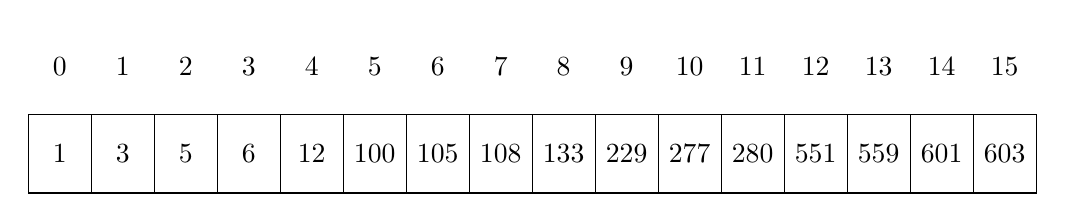
\begin{tikzpicture}[every node/.style={draw, minimum width=0.8cm, minimum height=1cm, anchor=west}]
    % Array elements (values)
    \foreach [count=\n from 0] \i in {1, 3, 5, 6, 12, 100, 105, 108, 133, 229, 277, 280, 551, 559, 601, 603} {
        \node at (\n*0.8cm, 0) {\i};
    }

    % Array indices (labels)
    \foreach [count=\n from 0] \i in {0, 1, 2, 3, 4, 5, 6, 7, 8, 9, 10, 11, 12, 13, 14, 15} {
        \node[draw=none, anchor=west] at (\n*0.8cm, 1.1cm) {\i};
    }
\end{tikzpicture}
\end{center}

and new element $t=7$ and call Insert($A, t$). Draw the recursion tree for the resulting call to
InsertRecursive, labeling each node with the values of min and max for that call. The first node is
given for you.

\begin{center}
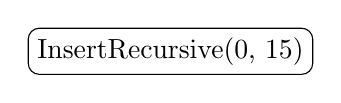
\begin{tikzpicture}
  \node[rectangle, draw, rounded corners] {InsertRecursive(0, 15)};
\end{tikzpicture}
\end{center}

\newpage


\item Describe a worst-case input for Insert, or explain why
all inputs take asymptotically the same time.
\vspace{1.5in}

\item 
What is the recurrence relation for the worst-case runtime of InsertRecursive on
an array of length $n$?

    \[
T(n) = 
\begin{cases} 
      1 & \text{if } n = 1\\
      \underline{\hspace{2in}} & \text{if } n > 1.
   \end{cases}
\]

\item What is the depth of the recursion tree for an input array of length $n$?
\vspace{1in}

\item What is work done at each node?
\vspace{1in}

\item Give a function $f(n)$ such that the worst-case runtime of
InsertRecursive is $\Theta(f(n))$.


\newpage

% Source: cs332-fall2025/exams/exam2_practice2/main.tex
\subsection*{From Fall 2025 Exam 2 Practice 2}
In this section, we will think about the computational problem of where to
insert a new element into a sorted array. Specifically, we will return the
position \emph{after which} to insert the element. For example, in the array
$A=[5, 40, 44, 600]$, we would insert the element $41$ after index $1$. If we
need to insert the new element before the current first element, we return $-1$.

\item Let $A=[-85, -45, -5, 6, 12, 18]$. After which index would we insert a new
element $15$? (You only get points if you give an index here, not ``between x
and y" or something similar.) Assume the indices start at $0$.

\vspace{1in}

\item Give a naive, $\Theta(n)$ worst-case time algorithm to solve the Insert
problem. Remember to return the index after which to insert the new element.

\begin{algo}
    NaiveInsert(sorted array $A$, new element $t$):\+\\[2in]
    \hspace{5in}

\end{algo}



\item We can solve this problem using divide and conquer based on the following
observation: given a sorted array $A$ and a new element $t$, the index after
which to insert $t$ must either occur in (fill in the blanks):
\begin{itemize}
    \item \underline{\hspace{4in}}, or
    \item \underline{\hspace{4in}}
\end{itemize}

\newpage

The pseudocode to implement a divide-and-conquer Insert is shown below. Recall
that $\lfloor x \rfloor$ takes the \emph{floor} of $x$, meaning that it rounds
down to the nearest integer.

\begin{algo}
    Insert(sorted array $A$, new element $t$):\+\\
    min = 0\\
    max = length of $A$ - 1\\
    make $A$ and $t$ global\\
    return InsertRecursive(min, max)
\end{algo}

\begin{algo}
    InsertRecursive(index min, index max):\+\\
    If min = max:\+\\
    If $t < A[$min]:\+\\
    Return min -1\-\\
    Else:\+\\
    Return min\-\-\\
    Else:\+\\
    mid = $\lfloor$ (min + max) / 2 $\rfloor$\\
    If $t < A$[mid]:\+\\
    return InsertRecursive(min, mid - 1)\-\\
    Else:\+\\
    return InsertRecursive(mid + 1, max)
\end{algo}

\item Suppose you have the length 16 array $A$ below, with indices
labeled above the array entries:

\begin{center}
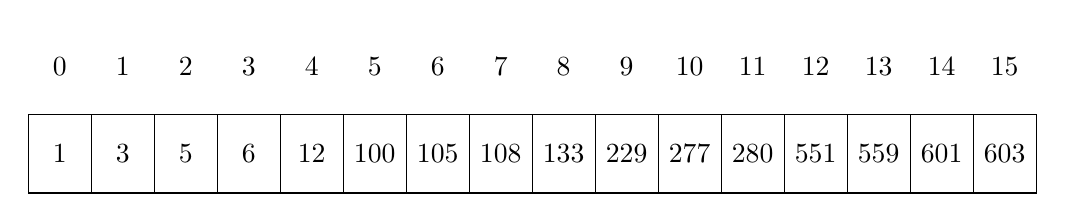
\begin{tikzpicture}[every node/.style={draw, minimum width=0.8cm, minimum height=1cm, anchor=west}]
    % Array elements (values)
    \foreach [count=\n from 0] \i in {1, 3, 5, 6, 12, 100, 105, 108, 133, 229, 277, 280, 551, 559, 601, 603} {
        \node at (\n*0.8cm, 0) {\i};
    }

    % Array indices (labels)
    \foreach [count=\n from 0] \i in {0, 1, 2, 3, 4, 5, 6, 7, 8, 9, 10, 11, 12, 13, 14, 15} {
        \node[draw=none, anchor=west] at (\n*0.8cm, 1.1cm) {\i};
    }
\end{tikzpicture}
\end{center}

and new element $t=7$ and call Insert($A, t$). Draw the recursion tree for the resulting call to
InsertRecursive, labeling each node with the values of min and max for that call. The first node is
given for you.

\begin{center}
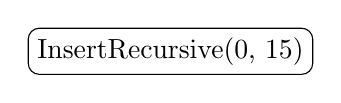
\begin{tikzpicture}
  \node[rectangle, draw, rounded corners] {InsertRecursive(0, 15)};
\end{tikzpicture}
\end{center}

\newpage


\item Describe a worst-case input for Insert, or explain why
all inputs take asymptotically the same time.
\vspace{1.5in}

\item 
What is the recurrence relation for the worst-case runtime of InsertRecursive on
an array of length $n$?

    \[
T(n) = 
\begin{cases} 
      1 & \text{if } n = 1\\
      \underline{\hspace{2in}} & \text{if } n > 1.
   \end{cases}
\]

\item What is the depth of the recursion tree for an input array of length $n$?
\vspace{1in}

\item What is work done at each node?
\vspace{1in}

\item Give a function $f(n)$ such that the worst-case runtime of
InsertRecursive is $\Theta(f(n))$.



\newpage
% Source: cs332-fall2025/exams/final/sections/divide_and_conquer.tex
\subsection*{From Fall 2025 Final Exam}

\item Given the following (meaningless) divide and conquer algorithm,
what is the recurrence relation that describes its runtime?
Notice the $n$ is the number of rows and the number of columns in the square array $A$,
not the total number of elements.

    \begin{algo}
    hi(square array $A$ of with $n$ rows and $n$ columns): \+ \\
    if $n = 1$:\+\\
        return $sum(A)$\-\\
    else:\+\\
    Let $A_1, A_2, A_3, A_4$ be the upper left, upper right, lower left, and lower right of $A$\\
    $X_1$ = hi($A_1$ + $A_4$)\\
    $X_2$ = hi($A_2$ + $A_3$)\\
    $C$ = $X_1$ + $X_2$\\
    return $C$\-\\
    \end{algo}

\begin{enumerate}[A.]
    \item $T(n) = 2T(n^2/2) + \Theta(n^2)$
    \item $T(n) = T(n/2) + \Theta(n^2)$
    \item $T(n) = 2T(n/2) + \Theta(n^2)$
    \item $T(n) = 2T(n/2) + \Theta(n)$
    \item $T(n) = 2T(n-2) + \Theta(n^2)$
\end{enumerate}

\item[] The next two questions refer to the recurrence relation
\[T(n) = 3T(n/4) + \Theta(n^2).
\]
\item What is the work done at each level of the recursion tree for this recurrence?
\begin{enumerate}[A.]
    \item $3^{\ell} + n^2$
    \item $3^{\ell} \left(\frac{n}{4^\ell}\right)^2$
    \item $\frac{4}{3} \ell^n$
    \item $n^2/4 + 3^\ell$
    \item $\frac{\ell \cdot n^2}{3}$
\end{enumerate}

\item How many levels does the recursion tree have?

\begin{enumerate}[A.]
    \item $\log_4 n$
    \item $\log_3 n$
    \item $n$
    \item $^3\sqrt{n}$
    \item $n \log_3 4$

\end{enumerate}

\item[]

The following questions refer to the problem of multiplying two n-digit
numbers.

\item Below is a divide and conquer algorithm to multiply two n-digit numbers $x$
and $y$ based on the observation that, if $a$ and $b$ are the first and second halves
of $x$ and $c$, and $d$ are the first and second halves of $y$ respectively, then

\[
x \cdot y = 10^n \cdot a \cdot c + 10^{n/2} \cdot (a \cdot d + b \cdot c) + b \cdot d.
\]

    \begin{algo}
    Split-Multiply(length $n$ integers $x$, $y$):\+\\
    \# base case\\
    if $n = 1$:\+\\
        return \underline{\hspace{1in}}\- \\
    \\
    \# recursive case\\
    else:\+\\
    Split $x$ into two halves $a$ and $b$\\
    Split $y$ into two halves $c$ and $d$\\
    $m=n/2$\\
    $e = $ Split-Multiply($a$, $c$) \\
    $f = $ Split-Multiply($b$, $d$) \\
    $g = $ Split-Multiply($b$, $c$) \\
    $h = $ Split-Multiply($a$, $d$) \\
    return $10^{2m} \cdot e + 10^{m} \cdot (g + h) + f$
    \end{algo} 

What should be returned in the base case (the blank above)?
\begin{enumerate}[A.]
    \item $0$
    \item $1$
    \item $x + y$
    \item $x \cdot y$
    \item $x - y$
\end{enumerate}

\item If $x=1234$ and $y=5678$, what are the values of $a$, $b$, $c$, and $d$ when
Split-Multiply($x,y,4$) is called?
\begin{enumerate}[A.]
    \item $a=12$, $b=34$, $c=56$, $d=78$
    \item $a=1$, $b=234$, $c=5$, $d=678$
    \item $a=123$, $b=4$, $c=567$, $d=8$
    \item $a=1234$, $b=0$, $c=5678$, $d=0$
    \item $a=0$, $b=1234$, $c=0$, $d=5678$  
\end{enumerate}

\item What is the runtime of Split-Multiply as a function of $n$, the number of digits
in the input numbers $x$ and $y$?
\begin{enumerate}[A.]
    \item $\Theta(n)$
    \item $\Theta(n \log n)$
    \item $\Theta(n^2)$
    \item $\Theta(n^{\log_2 3})$
    \item $\Theta(2^n)$
\end{enumerate}
\newpage

\begin{center}
\LARGE\textbf{Section 4 (1D Dynamic Programming)\\}%
\end{center}

% Source: cs332-fall2025/exams/exam2/main.tex
\subsection*{From Fall 2025 Exam 2}
\item (10 points) Given the following (meaningless) recursive definition of a subproblem, draw the 
recursion tree for a call to $huh(5)$ with each node labeled with the value of the argument to $huh$.

\begin{equation*}
    huh(i) =
    \begin{cases}
        4 & if i = 1 \\
        -100 & if i = 2\\
        0 & if i = 3\\
        \min \left(2 + huh(i-1), huh(i-3)\right) & if i > 3 \\

    \end{cases}
\end{equation*}

The first node is provided for you.

\begin{center}
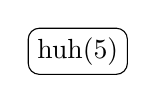
\begin{tikzpicture}
  \node[rectangle, draw, rounded corners] {huh(5)};
\end{tikzpicture}
\end{center}

\newpage

    \item (5 points)
    In this problem, you will need to write the English definition
    for the subproblem (step one of our four steps for writing dynamic programming algorithms)
    for the following problem.
    
    \textbf{The problem.} In order to cross the river, you need to hop from stone to stone.
    There are a total of $n$ stones in a line, each with height $h_i$. You can only jump
    from stone $i$ to stone $i+1$ or stone $i+2$.
    To conserve energy, you want to minimize the total vertical distance that
    you jump (both up and down). That is, if you jump from stone $i$ to stone $j$,
    you have covered $|h_i - h_j|$ vertical distance. What is the minimum total
    vertical distance needed to jump from stone 1 to stone n?

    To solve this problem, we first write the English definition of the subproblems we will solve.

    \textbf{1. The subproblem.} Let \underline{\hspace{10cm}}
    \underline{\hspace{14cm}}.



    \item (10 points)
    In this problem, you will need to write the formal recursive definition
    for the subproblem (step two of our four steps for writing dynamic programming algorithms)
    for the following problem.
    
    \textbf{The problem.} In your country, there are only coins of denominations
    1, 3, and 4. Given a pasitive integer n, what is the fewest number of
    coins you can use to represent n?

    To solve this problem, we first write the English definition of the subproblem.

    \textbf{1. The subproblem.} Let $MinCoins(i)$ be the minimum number of coins needed to represent the amount $i$.

    Next, we think about the recursive relationship between subproblems. You notice that in order to make $i$,
    you could either have made $i-1$ and added a 1-coin, or made $i-3$ and added a 3-coin,
    or made $i-4$ and added a 4-coin. Using this observation, fill in the formal recursive
    definition for $MinCoins(i)$ below.

    \textbf{2. The recursive definition.} The recursive relationship can be expressed as:
    (fill in both recursive case(s) and base case(s). You may not need every line provided!)

    \begin{equation*}
        MinCoins(i) =
        \begin{cases}
        \underline{\hspace{3in}} & if i \underline{\hspace{1in}} \\
        \underline{\hspace{3in}} & if i \underline{\hspace{1in}} \\
        \underline{\hspace{3in}} & if i \underline{\hspace{1in}} \\
        \underline{\hspace{3in}} & if i \underline{\hspace{1in}} \\
        \underline{\hspace{3in}} & if i \underline{\hspace{1in}} \\
        \end{cases}
    \end{equation*}

    \item (10 points) In this problem, you will need to write algorithm pseudocode  
    (step four of our four steps for writing dynamic programming algorithms)
    for the following problem.

\textbf{The problem} Having spied some snow on the mountains, you are thinking
about ski season. You would like to choose a ski jumping course that allows for
the maximum total distance in the air. The input to your problem is a set of $n$
jumps at positions $s_1, s_2, \ldots, s_n$ on the slope along with jump
distances $d_1, d_2, \ldots, d_n$ which indicate how far each jump will send
you. Some jumps may launch you over other jumps, but you can assume that you can
always land safely and complete the next jump. Let $p_i$ be the farthest along jump
that does not conflict with jump $i$ (i.e., the farthest along jump you could have
taken and still landed safely before jump $i$). If no such jump exists, let $p_i = 0$.

To solve this problem, we first write the English definition of the subproblems.

    \textbf{1. The subproblem.} Let $MaxAir(i)$ be the maximum distance you can jump,
    assuming you only consider jumps $1$ through $i$.

    Next, we think about the recursive relationship between subproblems.  You
    notice that if you take the $i$th jump, you get $d_i$ distance, but you can only use
    jumps 1 through $p_i$. If you don't take the $i$th jump, then you can use jumps
    1 through $i-1$. Using this observation, you write the formal recursive definition for
    $MaxAir(i)$ as follows.

    \textbf{2. The recursive definition.} 

    \begin{equation*}
        MaxAir(i) =
        \begin{cases}
            0 & if i = n \\
            max(d_i + MaxAir(p_i), MaxAir(i-1)) & if i < 0 \\

        \end{cases}
    \end{equation*}

    \textbf{3. How to memoize.} We can use an array of length $n$ to store the values of $MaxAir(i)$
    and fill it in increasing order.


    \textbf{4. Write the algorithm.} Using the above information, finish the pseudocode
    to find the maximum amount of air you can get on the ski jumps,
    given $s[1..n], d[1..n]$, and $p[1..n]$.
    \begin{algo}
    SkiJump($s[1..n], d[1..n], p[1..n]$):\+\\
    Let array $A$ be an array of length $n$\\
    \# do we have any base cases?\\
    \\
    \\
    \\
    \\
    \\
    \# how should we fill in the rest of the array?\\
    \\
    \\
    \\
    \\
    \\
    \\
    \\
    \\
    \# what should we return to get the final answer?\\
    \\
    \\
    \\
    \hspace{5in}
    \end{algo}


\newpage

% Source: cs332-fall2025/exams/exam2_practice1/main.tex
\subsection*{From Fall 2025 Exam 2 Practice 1}
Recall the \emph{weighted interval scheduling problem} from class. In this
problem, we are given $n$ intervals, each with a start time $s(i)$, a finish
time $f(i)$, and a weight $w(i)$. The goal is to find a set of mutually
compatible intervals with maximum total weight.

We will also define $p(i)$ to be the index of the last interval that finishes
before interval $i$ starts (or $0$ if there is no such interval).

\item For the example below, fill in the values of $p(2)$ through $p(8)$.

\begin{center}
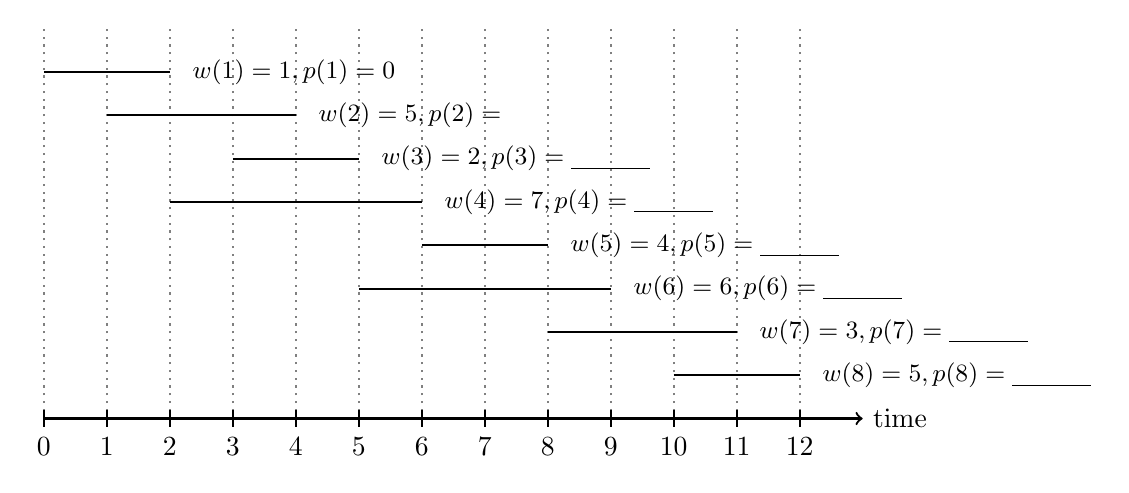
\begin{tikzpicture}[xscale=0.8, yscale=1.1, thick,
    interval/.style={draw, fill=blue!15, rounded corners=2pt, line width=0.8pt},
    label/.style={anchor=west, font=\small}]
    
    % x-axis
    \draw[->] (0,4) -- (13,4) node[right]{time};

    % tick marks and dotted gridlines
    \foreach \x in {0,1,...,12} {
        \draw[dotted, gray] (\x,4) -- (\x,8.5); % vertical dotted lines
        \draw (\x,4.1) -- (\x,3.9) node[below]{\x}; % ticks + labels
    }


    % intervals in order of finish time (top to bottom)
    % (start, end, y, name, weight)
    \draw[interval] (0,8) -- (2,8);
    \node[label] at (2.2,8) {$w(1) = 1, p(1) = 0$};

    \draw[interval] (1,7.5) -- (4,7.5);
    \node[label] at (4.2,7.5) {$w(2) = 5, p(2) = $};

    \draw[interval] (3,7) -- (5,7);
    \node[label] at (5.2,7) {$w(3) = 2, p(3) = \underline{\hspace{1cm}}$};

    \draw[interval] (2,6.5) -- (6,6.5);
    \node[label] at (6.2,6.5) {$w(4) = 7, p(4) = \underline{\hspace{1cm}}$};

    \draw[interval] (6,6) -- (8,6);
    \node[label] at (8.2,6) {$w(5) = 4, p(5) = \underline{\hspace{1cm}}$};

    \draw[interval] (5,5.5) -- (9,5.5);
    \node[label] at (9.2,5.5) {$w(6) = 6, p(6) = \underline{\hspace{1cm}}$};

    \draw[interval] (8,5) -- (11,5);
    \node[label] at (11.2,5) {$w(7) = 3, p(7) = \underline{\hspace{1cm}}$};

    \draw[interval] (10,4.5) -- (12,4.5);
    \node[label] at (12.2,4.5) {$w(8) = 5, p(8) = \underline{\hspace{1cm}}$};
\end{tikzpicture}
\end{center}


In order to give a dynamic programming solution to this problem, we follow the
four steps:

\item English description of the subproblems:
\\
Let $MaxWeight(i)$ be the \underline{\hspace{3.9in}}\\
\underline{\hspace{5.6in}}.

\item

You notice that the maximum weight of any set of compatible intervals 
at index $i$ either:
\begin{itemize}
    \item does not include interval $i$, so the maximum weight is just the maximum weight
    up to $i-1$, or
    \item does include interval $i$, so the maximum weight is the weight of interval $i$
    plus the maximum weight up to $p(i)$.
\end{itemize}

Using this observation, fill in the recursive part of the recursive definition
of the subproblem with the notation provided for $w$ and $p$ values.
    \begin{equation*}
        MaxWeight(i) =
        \begin{cases}
        0 & if i = 0 \\
        \underline{\hspace{3in}} & if i > 0 \\
        \end{cases}
    \end{equation*}

\item To memoize this algorithm, we will use an array $A$ of length
\underline{\hspace{1in}} (be careful! only exact answers will get full credit)
to store the needed values of $MaxWeight(i)$ and fill it in increasing order.

\item Finally, we write the pseudocode for the algorithm using the above information.
Use an array $A$ to store the values of $MaxWeight(i)$. Assume that your
inputs are sorted by finishing time already.


   \begin{algo}
    MaxIntervalWeight($s[1..n], f[1..n], w[1..n], p[1..n]$):\+\\
    \# initialize an array A\\
    \\
    \\
    \\
    \# do we have any base cases?\\
    \\
    \\
    \\
    \\
    \\
    \# how should we fill in the rest of the array?\\
    \\
    \\
    \\
    \\
    \\
    \\
    \\
    \\
    \# what should we return to get the final answer?\\
    \\
    \\
    \\
    \hspace{5in}
    \end{algo}

\item What are the values of $A$ after running MaxIntervalWeight on the example above?


\newpage

% Source: cs332-fall2025/exams/exam2_practice2/main.tex
\subsection*{From Fall 2025 Exam 2 Practice 2}
Recall the \emph{weighted interval scheduling problem} from class. In this
problem, we are given $n$ intervals, each with a start time $s(i)$, a finish
time $f(i)$, and a weight $w(i)$. The goal is to find a set of mutually
compatible intervals with maximum total weight.

We will also define $p(i)$ to be the index of the last interval that finishes
before interval $i$ starts (or $0$ if there is no such interval).

\item For the example below, fill in the values of $p(3)$ through $p(8)$.

\begin{center}
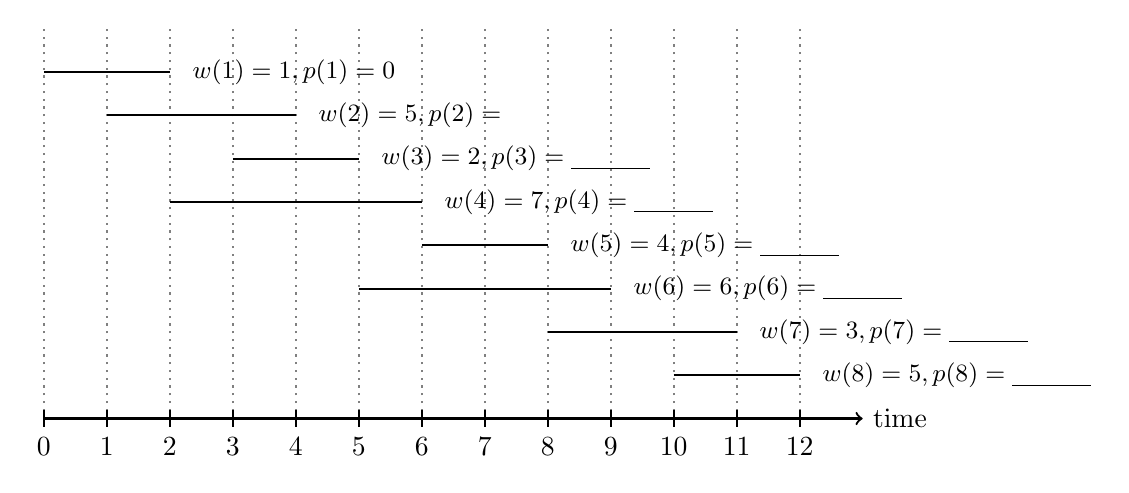
\begin{tikzpicture}[xscale=0.8, yscale=1.1, thick,
    interval/.style={draw, fill=blue!15, rounded corners=2pt, line width=0.8pt},
    label/.style={anchor=west, font=\small}]
    
    % x-axis
    \draw[->] (0,4) -- (13,4) node[right]{time};

    % tick marks and dotted gridlines
    \foreach \x in {0,1,...,12} {
        \draw[dotted, gray] (\x,4) -- (\x,8.5); % vertical dotted lines
        \draw (\x,4.1) -- (\x,3.9) node[below]{\x}; % ticks + labels
    }


    % intervals in order of finish time (top to bottom)
    % (start, end, y, name, weight)
    \draw[interval] (0,8) -- (2,8);
    \node[label] at (2.2,8) {$w(1) = 1, p(1) = 0$};

    \draw[interval] (1,7.5) -- (4,7.5);
    \node[label] at (4.2,7.5) {$w(2) = 5, p(2) = $};

    \draw[interval] (3,7) -- (5,7);
    \node[label] at (5.2,7) {$w(3) = 2, p(3) = \underline{\hspace{1cm}}$};

    \draw[interval] (2,6.5) -- (6,6.5);
    \node[label] at (6.2,6.5) {$w(4) = 7, p(4) = \underline{\hspace{1cm}}$};

    \draw[interval] (6,6) -- (8,6);
    \node[label] at (8.2,6) {$w(5) = 4, p(5) = \underline{\hspace{1cm}}$};

    \draw[interval] (5,5.5) -- (9,5.5);
    \node[label] at (9.2,5.5) {$w(6) = 6, p(6) = \underline{\hspace{1cm}}$};

    \draw[interval] (8,5) -- (11,5);
    \node[label] at (11.2,5) {$w(7) = 3, p(7) = \underline{\hspace{1cm}}$};

    \draw[interval] (10,4.5) -- (12,4.5);
    \node[label] at (12.2,4.5) {$w(8) = 5, p(8) = \underline{\hspace{1cm}}$};
\end{tikzpicture}
\end{center}


In order to give a dynamic programming solution to this problem, we follow the
four steps:

\item English description of the subproblems:
\\
Let $MaxWeight(i)$ be the \underline{\hspace{3.9in}}\\
\underline{\hspace{5.6in}}.

\item

You notice that the maximum weight of any set of compatible intervals 
at index $i$ either:
\begin{itemize}
    \item does not include interval $i$, so the maximum weight is just the maximum weight
    up to $i-1$, or
    \item does include interval $i$, so the maximum weight is the weight of interval $i$
    plus the maximum weight up to $p(i)$.
\end{itemize}

Using this observation, fill in the recursive part of the recursive definition
of the subproblem with the notation provided for $w$ and $p$ values.
    \begin{equation*}
        MaxWeight(i) =
        \begin{cases}
        0 & if i = 0 \\
        \underline{\hspace{3in}} & if i > 0 \\
        \end{cases}
    \end{equation*}

\item To memoize this algorithm, we will use an array $A$ of length
\underline{\hspace{1in}} (be careful! only exact answers will get full credit)
to store the needed values of $MaxWeight(i)$ and fill it in increasing order.

\item Finally, we write the pseudocode for the algorithm using the above information.
Use an array $A$ to store the values of $MaxWeight(i)$. Assume that your
inputs are sorted by finishing time already.


   \begin{algo}
    MaxIntervalWeight($s[1..n], f[1..n], w[1..n], p[1..n]$):\+\\
    \# initialize an array A\\
    \\
    \\
    \\
    \# do we have any base cases?\\
    \\
    \\
    \\
    \\
    \\
    \# how should we fill in the rest of the array?\\
    \\
    \\
    \\
    \\
    \\
    \\
    \\
    \\
    \# what should we return to get the final answer?\\
    \\
    \\
    \\
    \hspace{5in}
    \end{algo}

\item What are the values of $A$ after running MaxIntervalWeight on the example above?



\newpage
% Source: cs332-fall2025/exams/final/sections/dynamic_programming.tex
\subsection*{From Fall 2025 Final Exam}

\item[] The next three questions relate to the following problem:

In preparation for the University of Montana CS department's annual winter bowling party
(6-7:30pm this Saturday, December 13th, 2025 at Westside Lanes), you have been practicing with the following, simpler
version of bowling. There are $n$ pins in a single row, numbered from 1 to $n$.
Each pin $i$ has a point value $P[i]$ associated with it. You can knock down either one single pin
or two adjacent pins each time you roll the ball. Because you have been practicing so much, you
always hit the pins you aim for.
If you knock down pin $i$, you earn $P[i]$ points. If you knock down pins $i$ and $i+1$,
you earn the product $P[i] \cdot P[i+1]$ points.

You want to maximize your score by choosing which pins to knock down.

For example, if you have 4 pins with values $P=[2,3,5,1]$, one optimal strategy is to knock down pin 1 alone,
pins 2 and 3 together, and pin 4 alone, earning $2 + (3 \cdot 5) + 1 = 18$ points.

\item If you formulate subproblems for this bowling problem as \emph{Let $MaxPoints(i)$
be the maximum points you can earn by knocking down pins from $i$ to $n$},
how will you compute your final answer?
\begin{enumerate}[A.]
    \item $MaxPoints(1)$
    \item $MaxPoints(n)$
    \item $MaxPoints(MaxPoints)$
    \item $MaxPoints(1,n)$
    \item $MaxPoints(n,n)$
\end{enumerate}

\item If you formulate subproblems for this bowling problem as \emph{Let $MaxPoints(i)$
be the maximum points you can earn by knocking down pins from $1$ to $i$},
how will you compute your final answer?
\begin{enumerate}[A.]
    \item $MaxPoints(1)$
    \item $MaxPoints(n)$
    \item $MaxPoints(MaxPoints)$
    \item $MaxPoints(1,n)$
    \item $MaxPoints(n,n)$
\end{enumerate}

\item If you formulate subproblems for this bowling problem as \emph{Let $MaxPoints(i)$
be the maximum points you can earn by knocking down pins from $1$ to $i$},
which of the following is a correct recurrence relation for $MaxPoints(i)$?
\begin{enumerate}[A.]
    \item $MaxPoints(i) = \max \{ P[i] + MaxPoints(i-1), P[i] \cdot P[i+1] + MaxPoints(i+2) \}$
    \item $MaxPoints(i) = \max \{ P[i] + MaxPoints(i-1), P[i] \cdot P[i-1] + MaxPoints(i-2) \}$
    \item $MaxPoints(i) = \max \{ MaxPoints(i-1), MaxPoints(i-2) \}$
    \item $MaxPoints(i) = \max \{ P[i], P[i] \cdot P[i-1] \}$
    \item None of the above

\end{enumerate}
\end{enumerate}
\end{document}
